\documentclass[a4paper, 12pt]{mwart}
\usepackage[12pt]{moresize}
\usepackage[T1]{fontenc}
\usepackage{lipsum}
\usepackage{graphicx}
\usepackage[polish]{babel}
\usepackage{array}
\usepackage{cmbright}
\usepackage{polski}
\usepackage{amsmath}
\usepackage{wrapfig}
\usepackage[table, xcdraw]{xcolor}

\usepackage[margin = 1.cm]{geometry}

\setlength{\parskip}{4pt}

\setlength{\intextsep}{4pt}

\begin{document}
\pagenumbering{gobble}
	\begin{titlepage}
		\begin{center}
			
\includegraphics[height = 0.6\textheight]{pictures/agh_znk_wbr_rgb_150ppi.jpg}

			\begin{HUGE}
				Metody Obliczeniowe
				i Planowanie Eksperymentu
				\vspace{0.8cm}

				\emph{Projekt 1 - Zadanie 9 - Wariant 1}
			\end{HUGE}

		\end{center}
		\begin{figure}[b]
			\begin{tabular}{m{4cm}l}
				Imię i nazwisko  & \textbf{Wojciech Brandt}\\
				Number albumu    & \textbf{401 841}\\
				Wydział          & \textbf{Inżynierii Mechanicznej i Robotyki}\\
				Kierunek         & \textbf{Mechanika i Budowa Maszyn}\\
				Grupa Projektowa & \textbf{CP01}
			\end{tabular}
		\end{figure}
	\end{titlepage}

	\section{Opis eksperymentu}
		Podmiotem eksperymentu jest zmiana temperatury powietrza w ciągu roku. Od tej
		temperatury zależy bowiem efektywność instalacji grzewczych wykorzystujących
		pompę ciepła.

		W celu wykonania eksperymentu przeprowadzono pomiary wykorzystując przygotowany
		program\\ \textbf{z09v01.exe}. Zgodnie z zaleceniami zadania, jako zakres pomiarowy
		eksperymentu głównego wykorzystano 365 dni, lub inaczej $ \left\langle 1;365 
		\right\rangle$. Wyniki pomiarów to temperatura powietrza, podawana w stopniach celsjusza.

		Dostępne w załącznikach są programy, w których znajdują się skrypty użyte podczas generacji
		danych:
		\begin{description}
			\item[config.py] Plik konfiguracyjny.
			\item[custom\_approx.py] Moduł zawierający własnoręcznie napisane funkcje aproksymacyjne,
				oraz funkcje służące do oceny ich przydatności.
			\item[custom\_statistics.py] Moduł zawierający funkcje służące do wyznaczania parametrów statystycznych.
			\item[final\_notebook.ipynb] Zeszyt Jupyter Notebooks, implementujący funkcje z powyżej wymienionych modułów
				w celu wyznaczania i wymieniania danych. 
		\end{description}

	\section{Badanie wstępne}
		\subsection{Ogólne zachowanie układu}
			W celu zbadania zachowania układu przeprowadzono szereg badań, z różnymi zakresami badanymi.

			Na początek przeprowadzono badania mające na celu uzyskanie wielu punktów w różnych 
			przedziałach czasowych. Ostatecznie w celu zaprezentowania ogólnego działania układu 
			wygenerowano zestaw danych w zalecanym zakresie czasu $\left< 1;365 \right>$ dni, 
			generując 20 równo rozłożonych punktów:

			\begin{table}[h]
				\center
				\begin{tabular}{|c|c||c|c||c|c||c|c|}
					\hline
					Czas [dni] & Temp. [°C] & Czas [dni] & Temp. [°C] & Czas [dni] & Temp. [°C] & Czas [dni] & Temp. [°C]\\ \hline \hline
					1        & 11.8902  & 20.1578  & 13.8429  &  39.3157 & 15.5230 & 58.4736  & 17.8125 \\ \hline
					77.6315  & 19.4006  & 96.7894  & 21.1582  & 115.9473 & 21.9841 & 135.1052 & 22.3592 \\ \hline 
					154.2631 & 22.3124  & 173.4210 & 21.1953  & 192.5789 & 20.0178 & 211.7368 & 18.4292 \\ \hline 
					230.8947 & 15.9471  & 250.0526 & 14.1009  & 269.2105 & 12.7434 & 288.3684 & 11.1467 \\ \hline 
					307.5263 & 10.8011  & 326.6842 & 10.7493  & 345.8421 & 10.7206 & 365      & 11.8595 \\ \hline
				\end{tabular}
				\caption{Otrzymane pomiary do eksperymentu właściwego}
				\label{tab:main}
			\end{table}

			\begin{figure}[h]
				\begin{center}
					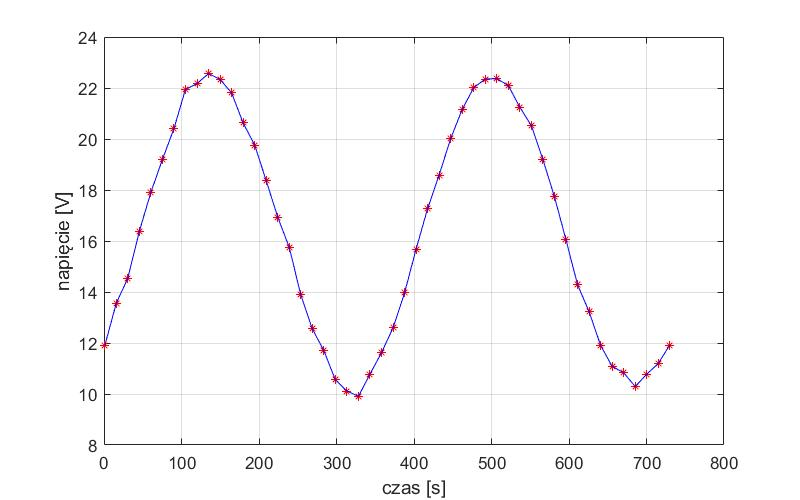
\includegraphics[width = 0.7\linewidth]{graphs/1A.jpg}
					\caption{Wykres danych z tabeli~\ref{tab:main}}
					\label{fig:1A}
				\end{center}
			\end{figure}

			Jak wydać na rys.~\ref{fig:1A} układ zachowuje się w taki sposób, że jego wykres w czasie wygląda 
			podobnie do wykresu funkcji sinusoidalnej. Na wykresie zaznaczone są punkty pomiarowe otrzymane 
			przy pomiarze (zaznaczone czerwonymi gwiazdkami).

			Z tab.~\ref{tab:main} i rys.~\ref{fig:1A} odczytać możemy istotne dane dla eksperymentu właściwego:
			\begin{itemize}
				\item Zakres badany: $\left< 1;365 \right>$
				\item Ilość węzłów: $20$
				\item Lokalne maksimum: $T_{max} = 22.3593 \text{ °C}$
				\item Lokalne minimum: $T_{min} = 10.7205 \text{ °C}$
				\item Wartość początkowa: $ T_{pocz} = 11.9803 \text{ °C}$
				\item Wartość końcowa: $ T_{kon} = 11.8595 \text{ °C}$ 
			\end{itemize}

		\subsection{Parametry statystyczne układu} \label{subsec:stats}
			
			W celu określenia istotnych parametrów statystycznych pomiaru, wykonano serię prób pomiarowych
			w tym samym punkcie czasowym. Powtórzeń wykonano 30, obrany punkt czasowy to $ T_{stat} = 170 \text{ dni} $

			\begin{table}[h]
				\center
				\begin{tabular}{|c|c||c|c||c|c||c|c||c|c||c|c|}
					\hline
					Lp. & Temp [°C] & Lp. & Temp [°C] & Lp. & Temp [°C] & Lp. & Temp [°C] & Lp. & Temp [°C]\\ \hline \hline
					1 & 21.3278 & 7 & 21.4407 & 13 & 21.5572 & 19 & 21.6734 & 25 & 21.8294 \\ \hline
					2 & 21.5581 & 8 & 21.5981 & 14 & 21.6125 & 20 & 21.6867 & 26 & 21.7179 \\ \hline
					3 & 21.6436 & 9 & 21.4865 & 15 & 21.7721 & 21 & 21.5976 & 27 & 21.4053 \\ \hline
					4 & 21.7363 & 10 & 21.3967 & 16 & 21.5016 & 22 & 21.8381 & 28 & 21.5411 \\ \hline
					5 & 21.7832 & 11 & 21.4783 & 17 & 21.5292 & 23 & 21.6015 & 29 & 21.6239 \\ \hline
					6 & 21.6631 & 12 & 21.7504 & 18 & 21.6604 & 24 & 21.4649 & 30 & 21.6096 \\ \hline
				\end{tabular}
				\caption{Dane otrzymane przy wielokrotnym mierzeniu w punkcie 170}
				\label{tab:stat}
			\end{table}

			\begin{wrapfigure}{r}{0.3\textwidth}	
				\begin{center}
					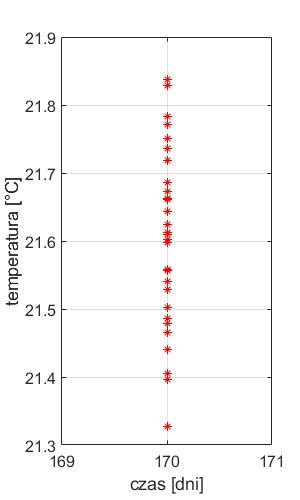
\includegraphics[width = 0.3\textwidth]{graphs/1C.jpg}
					\caption{Wykres danych z tab.~\ref{tab:stat}}
					\label{fig:stat}
				\end{center}
			\end{wrapfigure}

			Na podstawie danych z tab.~\ref{tab:stat} możemy wyznaczyć ważne wyznaczniki statystyczne
			dotyczące podmiotu badań.

			\begin{description}
				\item[Ilość powtórzeń] wynosi 30.
				\item[Średnia] wyznaczona na podstawie wzoru:
					$$ \bar{x} = \frac{1}{n} \sum_{i=1}^n x_i =  21.6028 \text{ °C}$$
			\end{description}

			\begin{description}
				\item[Wartość minimalna] $x_{min} = 21.3278 \text{ °C}$
				\item[Wartość maksymalna] $x_{max} = 21.8380 \text{ °C}$ 
				\item[Mediana] wynosi $21.5015 \text{ °C}$
				\item[Wariancja] wyznaczona na podstawie wzoru:
					$$ s^2 = \frac{1}{n - 1} \sum_{i=1}^n (y_i - \bar{y})^2 = 0.01713$$
				\item[Odchylenie standardowe] wyznaczone na podstawie wzoru:
					$$ s = \sqrt{\frac{1}{n - 1} \sum_{i=1}^n (y_i - \bar{y})^2} = 0.13089$$
			\newpage
				\item[Histogram]:
					\begin{figure}[h]
						\begin{center}
							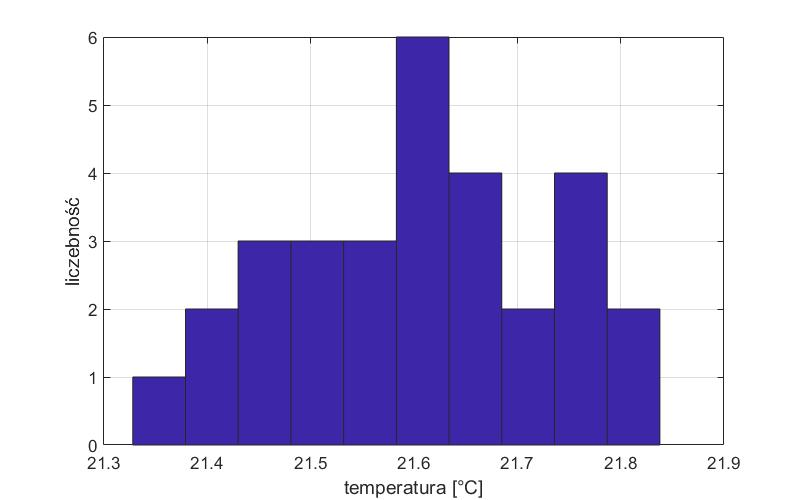
\includegraphics[width = 0.7\textwidth]{graphs/hist.jpg}
							\caption{Histogram oparty o dane z tab.~\ref{fig:stat}}
							\label{fig:hist}
						\end{center}
					\end{figure}
			\end{description}

			Aby dodatkowo sprawdzić rozkład pomiarów pod względem rozkładu, utworzono próbę zawierającą 
			100 powtórzeń:
			\begin{figure}[h]
				\begin{center}
					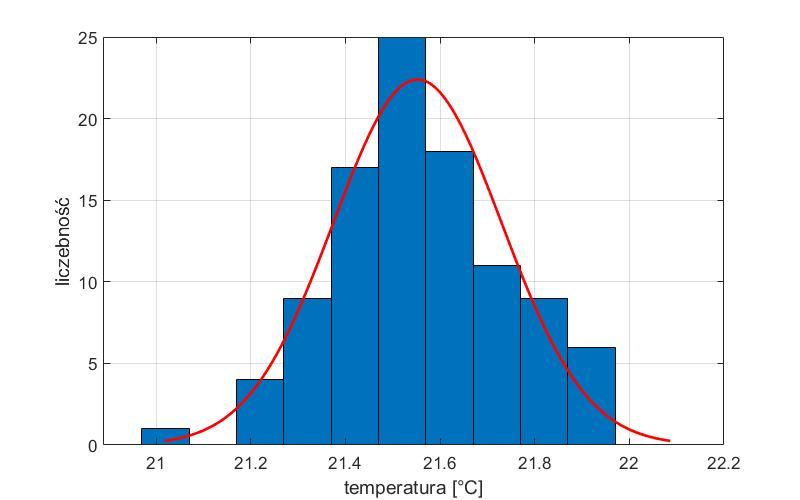
\includegraphics[width = 0.7\textwidth]{graphs/histfit.jpg}
					\caption{Histogram oparty o większą próbę, z dopasowanym rozkładem normalnym}
					\label{fig:histfit}
				\end{center}
			\end{figure}

			Sprawdzając dane przedstawione na rys.~\ref{fig:histfit} komputerowo pod kątem dopasowania 
			do rozkładu normalnego (m.in. wykonując test Shapiro-Wilka) otrzymujemy \emph{wartość p} na 
			poziomie 0.49, który jest większy od przyjętego poziomu istotności 0.05. Wynika z tego że 
			rozkład jest normalny.

	\newpage
	\section{Eksperyment właściwy}
		Następujące operacje przeprowadzane były na podstawie danych z tab.~\ref{tab:main}.

		\subsection{Standaryzacja zmiennych wejściowych}
			Pierwszym krokiem eksperymentu właściwego jest przeskalowanie (standaryzacja)
			danych do\\ przedziału $\left\langle -1; 1 \right\rangle$. Wykonano to za pomocą obliczenia:
			\begin{description}
				\item[średniej] ze wzoru:
					$$\bar{x} = \frac{x_{i,min} + x_{i,max}}{2}$$
				\item[jednostki zmienności] ze wzoru:
					$$\Delta x = \frac{x_{i,max} + x_{i,min}}{2}$$
				\item[Oraz podstawienia] powyższych wraz z kolejnymi wartościami $x_i$ do wzoru:
					$$t_i = \frac{x_i - \bar{x}}{\Delta x}$$
			\end{description}

			A więc dane z tab.~\ref{tab:main} przedstawione wobec nowej osi zmiennej standaryzowanej
			prezentują\\się następująco:
			\begin{figure}[h]
				\begin{center}
					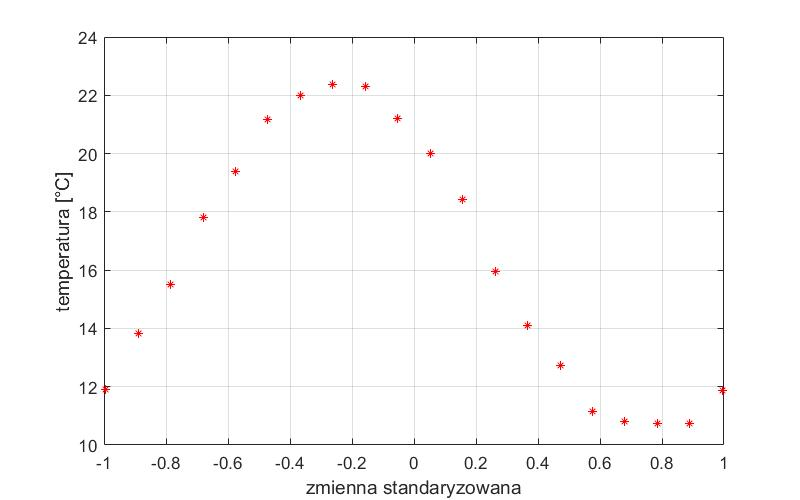
\includegraphics[width = 0.7\textwidth]{graphs/2B.jpg}
					\caption{Zmienne wejściowe przedstawione wobec osi $x$ standaryzowanej}
					\label{fig:2B}
				\end{center}
			\end{figure}

		\subsection{Opracowanie modelu badań}
			Model układu utworzony zostanie poprzez wykorzystanie aproksymacji średniokwadratowej.
			Uogólniony wzór funkcji aproksymującej wyglada w następujący sposób:
			$$ Q(x) = a_1 q_1(x) + a_2 q_2(x) + ... + a_j q_j(x) + ... a_m q_m(x) = \sum_{j=1}^m a_j q_x(x)$$
			gdzie $q_j(x)$ jest obraną funkcją bazową, a współczynniki $a_i$ wyznaczać będziemy ze
			wzoru macierzowego:
			$$ \textbf{A} = \left( \textbf{X}^T \cdot \textbf{X} \right)^{-1} \cdot \textbf{X}^T \cdot \textbf{Y} $$

			\subsubsection{Aproksymacja funkcją wielomianową}
				Wzór ogólny dla aproksymacji funkcjami wielomianowymi wygląda następująco:
				$$ Q(x) = a_1 + a_2x + a_3 x^2 + a_4 x^3 + \dots + a_n x^{n-1} $$
				
				I w celu określenia dobrego modelu dla układu można sprawdzać różne stopnie $n$, 
				na przykład $n=0$, co da nam funkcję stałej, $n=1$ co da nam prostą, $n=7$ co dam nam
				nam wielomian siódmego stopnia.

				Macierze aproksymacji wyglądać będą więc w następujący sposób:

				$$ \textbf{X} = \begin{bmatrix}
					1      & x_1    & \cdots & x_1^{n-1} \\
					1      & x_2    & \cdots & x_2^{n-1} \\
					\vdots & \vdots &        & \vdots\\ 
					1      & x_n    & \cdots & x_n^{n-1}
				\end{bmatrix} 
				\quad 
				\textbf{A} = \begin{bmatrix}
					a_1\\
					a_2\\
					\vdots\\
					a_n
				\end{bmatrix} \quad
				\textbf{Y} = \begin{bmatrix}
					y_1\\
					y_2\\
					\vdots\\
					y_n
				\end{bmatrix}$$

				\paragraph{Aproksymacja wielomianem 1-go stopnia}

					Otrzymana ze skryptu macierz $\textbf{A}$, wyliczona w oparciu o oś X wejściową:
					$$ \textbf{A} = \begin{bmatrix}
						19.6688 &
						-0.0189
					\end{bmatrix} $$

					Funkcja aproksymująca:
					$$ Q(x) = 19.6688 -0.0189x $$

					Otrzymana ze skryptu macierz $\textbf{B}$, wyliczona w oparciu o
					oś T standaryzowaną:
					$$ \textbf{B} = \begin{bmatrix}
						16.1997 &
						-3.4691
					\end{bmatrix} $$

					Funkcja aproksymująca:
					$$ Q(x) = 16.1997 -3.4691x$$

				\paragraph{Aproksymacja wielomianem 2-go stopnia}

					Otrzymana ze skryptu macierz $\textbf{A}$:
					$$\textbf{A} = \begin{bmatrix}
						13.8088 &
						0.0818 &
						-2.753 \cdot 10^{-4}
					\end{bmatrix}$$
					
					Funkcja aproksymująca: 
					$$ Q(x) = 13.8088 + 0.0818x -2.753 \cdot 10^{-4} \cdot x^2 $$

					Otrzymana ze skryptu macierz $\textbf{B}$:
					$$\textbf{B} = \begin{bmatrix}
						19.5594 &
						-3.4690 &
						-9.2197
					\end{bmatrix}$$

					Funkcja aproksymująca:
					$$ Q(x) = 19.5594 -3.4690x -9.2197x^2$$

				\paragraph{Aproksymacja wielomianem 7-go stopnia}

					Otrzymana ze skryptu macierz $\textbf{A}$:
					$$\textbf{A} = \begin{bmatrix}
						11.7930 &
						0.1012 &
						-2.88\cdot 10^{-4} &
						1.023\cdot 10^{-5} &
						-1.24\cdot 10^{-7} &
						5 \cdot 10^{-10} &
						0 &
						6.082
					\end{bmatrix}$$

					Funkcja aproksymująca (w przybliżeniu):
					$$ Q(x) \approx 11.7930 + 0.1012x + 6.082 x^7 $$

					Otrzymana ze skryptu macierz $\textbf{B}$:
					$$\textbf{B} = \begin{bmatrix}
						20.692 &
						-13.7 &
						-21.28 &
						24.59 &
						18.154 &
						-15.044 &
						-5.744 &
						4.180
					\end{bmatrix}$$

					Funkcja aproksymująca:
					$$ Q(x) = 20.692 - -13.7x -21.28x^2 + 24.59x^3 + 18.154x^4 - 15.044x^5 -5.744x^6 + 4.180x^7 $$

					\newpage
				\paragraph{Otrzymane funkcje} prezentują się w następujący sposób:

					Dla zmiennej wejściowej (na podstawie funkcji o współczynnikach macierzy $\textbf{A}$):
					\begin{figure}[h]
						\begin{center}
							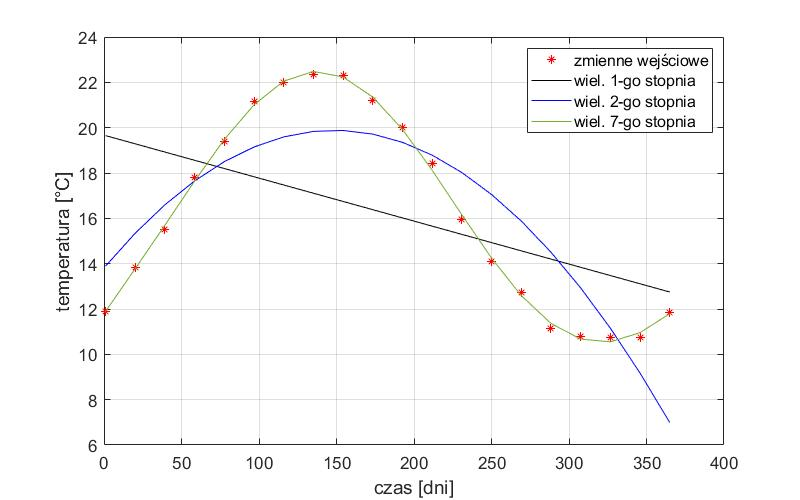
\includegraphics[width = 0.7\textwidth]{graphs/3-n.jpg}
							\caption{Wyniki aproksymacji wielomianami wobec osi zmiennych wejściowych}
							\label{fig:3N}
						\end{center}
					\end{figure}

					Dla zmiennej standaryzowanej (na podstawie funkcji o współczynnikach macierzy $\textbf{B}$):
					\begin{figure}[h]
						\begin{center}
							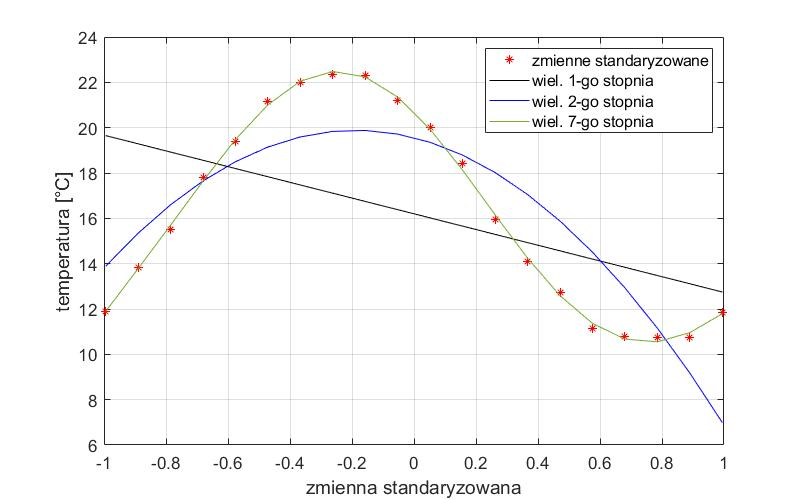
\includegraphics[width = 0.7\textwidth]{graphs/3-s.jpg}
							\caption{Wyniki aproksymacji wielomianami wobec osi zmiennych standaryzowanych}
							\label{fig:3S}
						\end{center}
					\end{figure}

			\subsubsection{Aproksymacja funkcją logarytmu naturalnego}
				Wzór uogólniony aproksymacji jest następujący:

				$$ Q(x) = a_1 + a_2 \ln\left(x\right) + a_3\ln^2\left(x\right) + \dots + a_n \ln^{n-1} \left(x\right)$$
			\newpage
				A macierze aproksymacji prezentują się w następujący sposób:
	
				$$ \textbf{X} = \begin{bmatrix}
					1      & \ln \left(x_1\right) & \cdots & \ln^{n-1} \left(x_1\right)\\
					1      & \ln \left(x_2\right) & \cdots & \ln^{n-1} \left(x_2\right)\\
					\vdots & \vdots               &        & \vdots \\
					1      & \ln \left(x_n\right) & \cdots & \ln^{n-1} \left(x_n\right)
				\end{bmatrix}
				\quad 
				\textbf{A} = \begin{bmatrix}
					a_1\\
					a_2\\
					\vdots\\
					a_n
				\end{bmatrix} \quad
				\textbf{Y} = \begin{bmatrix}
					y_1\\
					y_2\\
					\vdots\\
					y_n
				\end{bmatrix}$$	

				Na tym etapie należy zaznaczyć, że niemożliwe jest aproksymowanie funkcją logarytmu
				naturalnego w oparciu o zmienne standaryzowane, gdyż nie istnieje logarytm z wartości
				ujemnej.

				Macierz $\textbf{A}$ otrzymana ze skryptu:

				$$\textbf{A} = \begin{bmatrix}
					11.888\\
					286.226\\
					-267.589\\
					91.286\\
					-13.427\\
					0.719
				\end{bmatrix}$$

				A więc funkcja aproksymująca:
				$$Q(x) = 11.888 + 286.226 \ln \left(x\right) -267.589 \ln^2 \left(x\right)
				+ 91.286 \ln^3 \left(x\right) -13.427 \ln^4 \left(x\right) +0.719 \ln^5 \left(x\right)$$

				I jej wykres:
				\begin{figure}[h]
					\begin{center}
						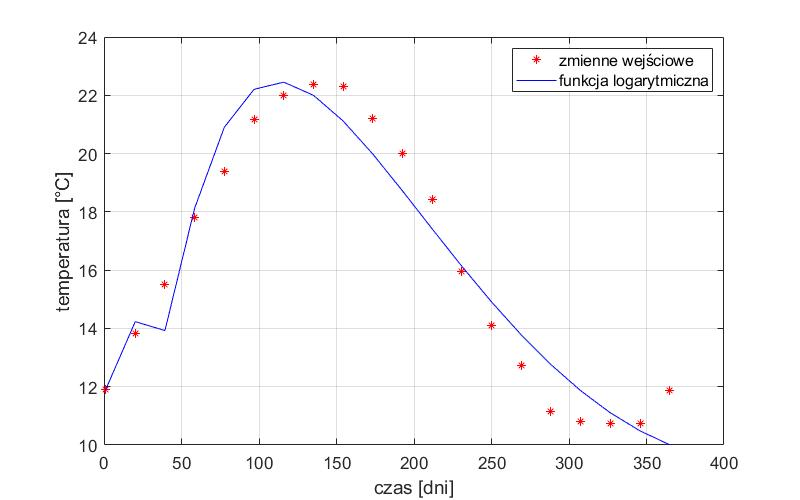
\includegraphics[width = 0.7\textwidth]{graphs/4-n.jpg}
					\end{center}
				\end{figure}

				Jak widać przy programowaniu skryptu zdecydowano się na przyjęcie stopnia $n=6$.
				Wybór ten wynika z nieadekwatności modelu do układu - dalsze zwiększanie współczynnika dawało
				niewiele lepsze rezultaty.

			\subsubsection{Aproksymacja funkcją wymierną}
				Wzór uogólniony funkcji jest następujący:
				$$Q(x) = a_1 + a_2 \left(\frac{1}{x}\right) + a_3 \left(\frac{1}{x}\right)^2 + \dots + a_n \left(\frac{1}{x}\right)^{n-1}$$

				A macierze aproksymujące są następujące:
				$$\textbf{X} = \begin{bmatrix}
					1     & \frac{1}{x_1} & \cdots & \left(\frac{1}{x_1}\right)^{n-1}\\
					1     & \frac{1}{x_2} & \cdots & \left(\frac{1}{x_2}\right)^{n-1}\\
					\vdots& \vdots        &        & \vdots\\
					1     & \frac{1}{x_n} & \cdots & \left(\frac{1}{x_n}\right)^{n-1}\\
				\end{bmatrix}
				\quad 
				\textbf{A} = \begin{bmatrix}
					a_1\\
					a_2\\
					\vdots\\
					a_n
				\end{bmatrix} \quad
				\textbf{Y} = \begin{bmatrix}
					y_1\\
					y_2\\
					\vdots\\
					y_n
				\end{bmatrix}$$

				Macierz $\textbf{A}$ otrzymana ze skryptu:
				$$\textbf{A} = \begin{bmatrix}
					-5.041 &
					7.142 \cdot 10^3 &
					-6.104 \cdot 10^5 &
					1.928 \cdot 10^7 &
					-2.052 \cdot 10^8 &
					1.865 \cdot 10^8
				\end{bmatrix}$$

				Funkcja aproksymująca:
				$$Q(x) = -5.041  + 7.142 \cdot 10^3 \cdot \frac{1}{x} -6.104 \cdot 10^5 \cdot
				\left(\frac{1}{x}\right)^2 +1.928 \cdot 10^7 \cdot \left(\frac{1}{x}\right)^3
				-2.052 \cdot 10^8 \cdot \left(\frac{1}{x}\right)^4 + 1.865 \cdot 10^8 \cdot \left(
				\frac{1}{x}\right)^5$$

				Macierz $\textbf{B}$ otrzymana ze skryptu:
				$$\textbf{B} = \begin{bmatrix}
					14.022 &
					-1.764 &
					0.213 &
					0.041 &
					-5.349 \cdot 10^{-4} &
					-9.925 \cdot 10^{-5}
				\end{bmatrix}$$
				
				Funkcja aproksymująca:
				$$Q(x) = 14.022
				-1.764\cdot \frac{1}{x} 
				+ 0.213\cdot \left(\frac{1}{x}\right)^2 
				+ 0.041\cdot \left(\frac{1}{x}\right)^3 
				-5.349\cdot 10^{-4}\cdot \left(\frac{1}{x}\right)^4   
				-9.925 \cdot 10^{-5}\cdot \left(\frac{1}{x}\right)^5$$

				Wykres funkcji aproksymującej na podstawie współczynników otrzymanych w oparciu
				o oś zmiennych wejściowych $\textbf{x}$:
				\begin{figure}[h]
					\begin{center}
						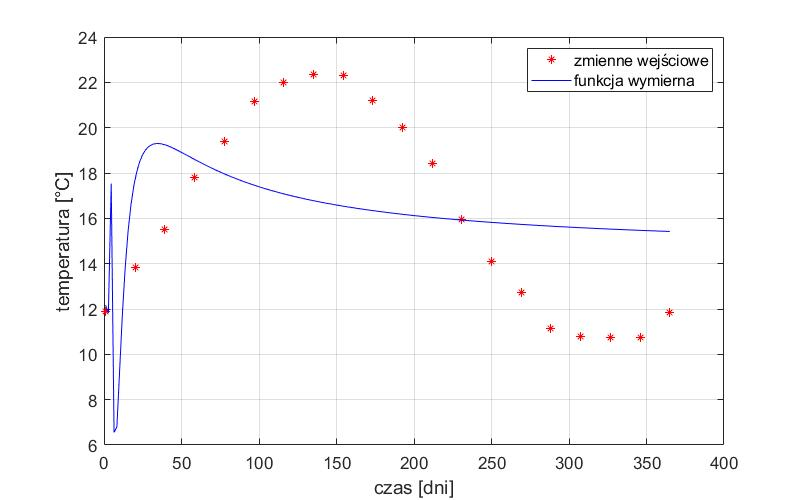
\includegraphics[width = 0.7\textwidth]{graphs/5-n.jpg}
						\caption{Wykres aproksymacji funkcją wymierną na zmiennych wejściowych}
						\label{fig:5n}
					\end{center}
				\end{figure}

				\newpage

				Wykres funkcji aproksymującej na podstawie współczynników otrzymanych w oparciu
				o oś zmiennych standaryzowanych $\textbf{t}$:
				\begin{figure}[h]
					\begin{center}
						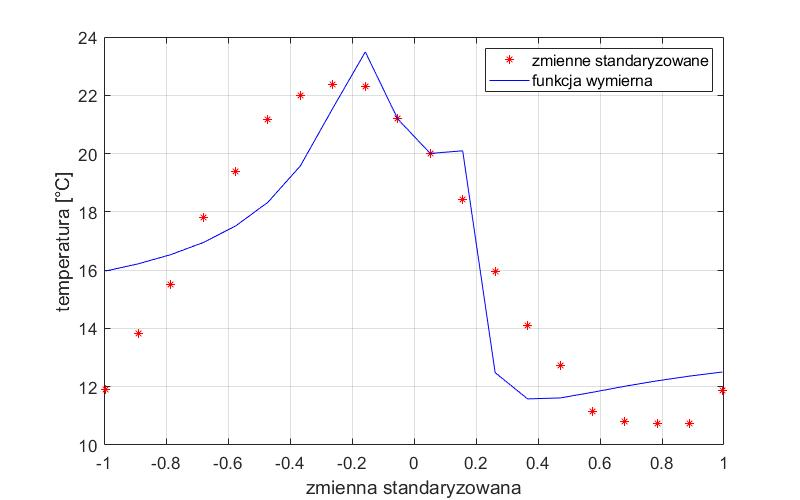
\includegraphics[width = 0.7\textwidth]{graphs/5-s.jpg}
						\caption{Wykres aproksymacji funkcją wymierną na zmiennych standaryzowanych}
						\label{fig:5s}
					\end{center}
				\end{figure}

			\subsubsection{Aproksymacja funkcją trygonometryczną}
				Wzór uogólniony wybranej funkcji ma następującą postać:
				$$Q(x) = a_1 + a_2 \cos(c\cdot x) + a_3 \sin (c\cdot x) + a_4 \cos(c\cdot 2x)
				+ a_5 \sin (c\cdot 2x) +\dots + a_n \cos (c\cdot \frac{n}{2}x) + 
				a_{n+1} \sin(c \cdot \frac{n}{2}x)$$

				Gdzie $c$ to zmienna mająca wpływ na okres funkcji aproksymowanej; podczas prób
				aproksymacji dobierana była empirycznie.

				Macierz aproksymacji $\textbf{X}$ przyjmie postać:
				$$\textbf{X} = \begin{bmatrix}
					1     & \cos(c\cdot x_1) & \sin(c\cdot x_1) & \cdots & \cos(c\cdot \frac{n}{2} x_1) & \cos(c\cdot \frac{n}{2} x_1)\\
					1     & \cos(c\cdot x_2) & \sin(c\cdot x_2) & \cdots & \cos(c\cdot \frac{n}{2} x_2) & \cos(c\cdot \frac{n}{2} x_2)\\
					\vdots& \vdots & \vdots &  & \vdots & \vdots\\
					1     & \cos(c\cdot x_n) & \sin(c\cdot x_n) & \cdots & \cos(c\cdot \frac{n}{2} x_n) & \cos(c\cdot \frac{n}{2} x_n)\\
				\end{bmatrix}$$

				Podczas aproksymacji w oparciu o zmienne wejściowe
				$x$ wybrano współczynnik $c=0.003\cdot \pi$. \\Macierz $\textbf{A}$ otrzymana ze skryptu:
				$$\textbf{A} = \begin{bmatrix}
					15.982 &
					-0.226 &
					0.579 &
					-3.923 &
					4.541
				\end{bmatrix}$$

				Postać funkcji aproksymującej:
				$$Q(x) = 15.982 -0.226 \cos\left(c\cdot x\right) + 0.579 \sin \left(c\cdot x\right)
				- 3.923 \cos \left(c\cdot 2x\right) + 4.541 \sin \left(c \cdot 2x\right)$$

				Podczas aproksymacji w oparciu o zmienne standaryzowane $t$ wybrano współczynnik 
				$c=\pi$. \\Macierz $\textbf{B}$ otrzymana ze skryptu:
				$$\textbf{B} = \begin{bmatrix}
					16.395 &
					4.316 &
					-4.218 &
					-0.047 &
					-0.0628
				\end{bmatrix}$$

				Postać funkcji aproksymującej:
				$$Q(x) = 16.395 + 4.316 \cos\left(c\cdot x\right) -4.218 \sin \left(c\cdot x\right)
				-0.047 \cos \left(c\cdot 2x\right) -0.0628 \sin \left(c \cdot 2x\right)$$
			\newpage

				Wykres funkcji aproksymującej na podstawie współczynników otrzymanych w oparciu
				o oś zmiennych wejściowych $x$:
				\begin{figure}[h]
					\begin{center}
						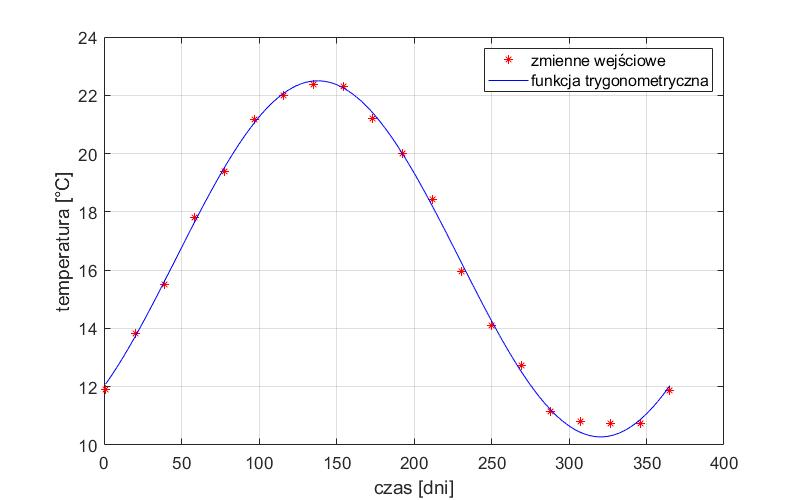
\includegraphics[width = 0.7\textwidth]{graphs/6-n.jpg}
						\caption{Wykres aproksymacji funkcją trygonometryczną na zmiennych wejściowych}
						\label{fig:6n}
					\end{center}
				\end{figure}

				Wykres funkcji aproksymującej na podstawie współczynników otrzymanych w oparciu
				o oś zmiennych standaryzowanych $t$:
				\begin{figure}[h]
					\begin{center}
						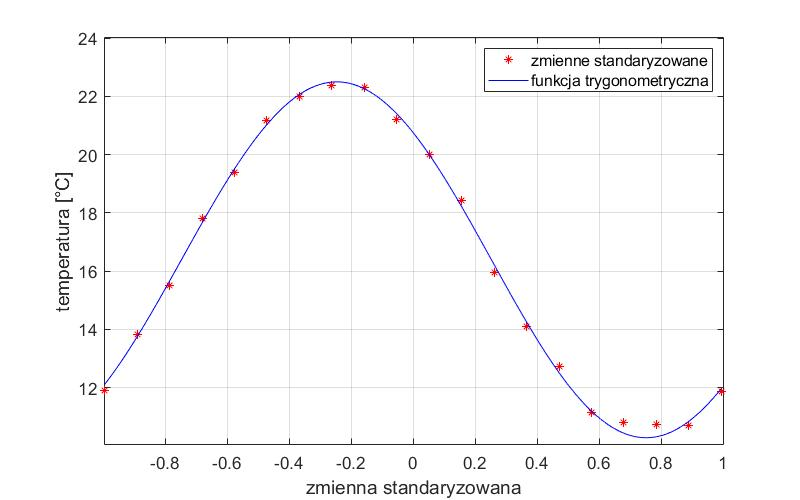
\includegraphics[width = 0.7\textwidth]{graphs/6-s.jpg}
						\caption{Wykres aproksymacji funkcją trygonometryczną na zmiennych standaryzowanych}
						\label{fig:6s}
					\end{center}
				\end{figure}

		\subsection{Ocena przydatności przyjętych modeli}
			\subsubsection{Ocena wizualna}
				Na podstawie oceny wizualnej od razu można ocenić, że najlepiej aproksymującymi modelami
				były te, które oparte były na funkcji wielomianu wysokiego stopnia oraz na funkcji
				trygonometrycznej. Pozostałe modele, nawet pomimo prób zwiększania ich stopnia $n$ (jak
				w przypadku funkcji wymiernej oraz logarytmicznej), nie
				dawały dobrych rezultatów. W związku z tym w dalszej części oceniana będzie zdatność modelu
				opartego o wielomian 7-go stopnia (przedstawiony na rys.~\ref{fig:3N} oraz na rys.~\ref{fig:3S}),
				oraz opartego o funkcję trygonometryczną (przedstawiony na rys.~\ref{fig:6n} oraz
				na rys. ~\ref{fig:6s}).
			
			\subsubsection{Wyznaczanie błędów oraz współczynników opisujących zdatnośc modelu}
				Do dokładniejszej, systematycznej oceny modelu wykorzystane zostaną następujące własności:

				\begin{description}
					\item[Błąd bezwzględny]: $$|\Delta y_i| = |\hat{y_i}-y_i|$$
					\item[Błąd względny]: $$|\varepsilon_i|=\frac{|\hat{y_i}-y_i|}{|y_i|}$$
					\item[Współczynnik determinancji $R^2$] wyznaczony na podstawie wzoru:
						$$ R^2 = 1-\frac{\displaystyle\sum_{i=1}^n \left(\hat{y_i} - y_i\right)^2}
						{\displaystyle\sum_{i=1}^n \left(y_i - \bar{y}\right)^2} $$ 
					\item[Pierwiastek błędu średniokwadratowego RMSE]:
						$$\text{RMSE} = \sqrt{\frac{1}{N} \sum_{i=1}^n (\hat{y_i} - y_i)^2}$$ 
				\end{description}

				Na tablicy~\ref{tab:err} przedstawione zostały obliczone własności modeli:
				\begin{enumerate}
					\item Wielomian 7-go stopnia wyznaczony na podstawie zmiennych wejściowych
					\item Wielomian 7-go stopnia wyznaczony na podstawie zmiennych standaryzowanych
					\item Funkcja trygonometryczna wyznaczona na podstawie zmiennych wejściowych
					\item Funkcja trygonometryczna wyznaczona na podstawie zmiennych standaryzowanych
				\end{enumerate}

				Wynikowe błędy względne i bezwzględne to średnie wartości wszystkich węzłów.
				\vspace{8pt}
				\begin{table}[h]
					\centering
					\begin{tabular}{c|c|c|c|c|}
						\cline{2-5}
						\cellcolor[HTML]{FFFFFF}              & 1.                     & 2.                     & 3.                     & 4.                     \\ \hline
						\multicolumn{1}{|c|}{$\Delta y_i$}    & $0.9502 \cdot 10^{-2}$ & $0.9502 \cdot 10^{-2}$ & $1.0461 \cdot 10^{-2}$ & $1.1412 \cdot 10^{-2}$ \\ \hline
						\multicolumn{1}{|c|}{$\varepsilon_i$} & $1.4070 \cdot 10^{-1}$ & $14070 \cdot 10^{-1}$ & $1.5119\cdot 10^{-1}$  & $1.6368 \cdot 10^{-1}$ \\ \hline
						\multicolumn{1}{|c|}{$R^2$}           & 0.9986                 & 0.9986                 & 0.9984                 & 0.9982                 \\ \hline
						\multicolumn{1}{|c|}{$RMSE$}          & 0.1573                 & 0.1573                 & 0.1705                 & 0.1773                 \\ \hline
					\end{tabular}
					\caption{Błędy oraz współczynniki adekwatności modeli}
					\label{tab:err}
				\end{table}

		\newpage				

		\subsection{Wnioski}

		Trudno stwierdzić który z modeli (wielomianowy czy  trygonometryczny) jest lepszy;
		z jednej strony wartości przedstawione
		w tabeli~\ref{tab:err} pokazują, że model oparty o wielomian 7-go stopnia jest dokładniejszy,
		jego błedy są mniejsze, współczynnik determinancji $R^2$ jest bliższy $1$ (im bliżej 
		$1$ tym lepsze dopasowanie), a błąd $RMSE$ jest mniejszy (im bliżej $0$ tym lepiej).
		Warto jednak zaznaczyć, że jest tak dla wybranego przedziału; gdyby wybrać szerszy przedział
		czasowy, na przykład $\left\langle 1; 2000 \right\rangle$, to bardzo szybko jego dokładność
		by spadła w porównaniu do modelu opartego o funkcje trygonometryczne, który w dalszym ciągu
		byłby dobrze dopasowany.

		\begin{figure}[h]
			\begin{center}
				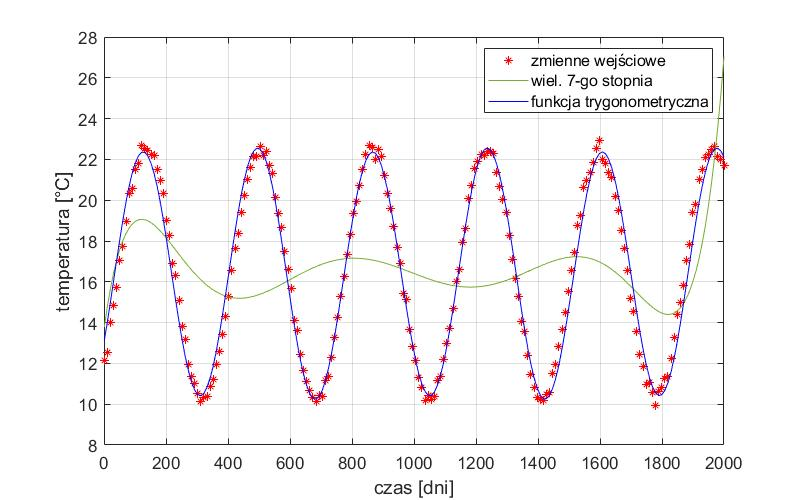
\includegraphics[width = 0.74\textwidth]{graphs/7.jpg}	
				\caption{Prezentacja działania modeli na dłuższym przedziale czasowym}
				\label{fig:7}
			\end{center}
		\end{figure}

		Jak widać na rys.~\ref{fig:7} model oparty o aproksymację trygonometryczną na dłuższym przedziale czasowym utrzymuje
		swoją zdatność, podczas gdy wielomianowy kompletnie ją traci - aby model oparty o wielomiany ponownie stał się 
		dokładny, trzeba byłoby znacznie zwiększyć stopień funkcji podstawowej, przy czym nigdy nie nastąpi sytuacja w której
		będzie on w stanie aproksymować działanie układu w czasie nieskończonym, podczas gdy trygonometryczny jak najbardziej
		może tak zadziałać.

		Różnica dokładności między tymi dwoma modelami - wielomianowym i trygonometrycznym - wynika z faktu, że w ogólnym
		rozrachunku model wielomianowy stara się jak najdokładniej przybliżyć dowolną funkcję (przez co "wychwytuje" ~
		niewielkie wachania w stosunku do prostej funkcji trygonometrycznej ukazane w podrozdziale~\ref{subsec:stats}), 
		podczas gdy model trygonometryczny bardziej ogólnie opisuje zachowanie układu. Inaczej ujmując wystarczyłoby ponownie
		uruchomić eksperyment w celu uzyskania nowych danych aby zauważyć niepomijalne różnice w zapisie funkcji wielomianowej,
		podczas gdy funkcja trygonometryczna pozostałaby podobna.

		Pozostałe modele nie dawały zadowalających wyników, różnice pomiędzy krzywą zakreślaną przez węzły a funkcjami logarytmiczną
		oraz wymierną były bardzo duże, zauważalne gołym okiem. Być może byłyby one dobrymi modelami dla innych układów/eksperymentów,
		lecz w tym nie sprawdziły się.
\end{document}